\section{Signal efficiency}\label{sec:WBoson_Efficiency}

The signal truth efficiency is estimated using the \WToMuNu\ NLO MC samples since they contain the full history of the events, including the generation and reconstruction of the particles. The energy deposited in the HF calorimeters is reweighed in MC to match the distribution observed in data as explained in \sect{sec:WBoson_Corrections_EventActivityReweighing}.

A reconstructed muon is considered an offline muon if it passes all the \W boson analysis cuts detailed in \sect{sec:WBoson_Selection_WSelection}. Among the selection criteria, an offline muon is required to pass the isolation and tight identification cuts defined in \sect{sec:WBoson_Selection_MuonIdentification}, be trigger matched, and have a $\pt~>~25$~\GeVc and $|\eta|~<~2.4$.

The muon truth efficiency is defined as the fraction of generated muons matched to an offline muon around a cone of $\Delta{R} < 0.05$.  All the generated muons are required to be inside the analysis kinematic region ($\pt~>~25$~\GeVc and $|\eta|~<~2.4$) and come from a \W boson decay. The muon truth efficiency is described in \eq{eq:MCTruthEfficiency}.

\begin{equation}
\epsilon^{\mu^{\pm}}_{offline}(p_{T}^{gen} , \eta^{gen}) = \frac{N_{gen,\pt>25}^{\mu^{\pm}}(p_{T}^{gen} , \eta^{gen})[\textnormal{Matched to }\mu_{offline}^{\pm}]}{N_{gen,\pt>25}^{\mu^{\pm}}(p_{T}^{gen} , \eta^{gen})}
\label{eq:MCTruthEfficiency}
\end{equation}

The muon efficiencies of the \RunpPb and \RunPbp MC samples are calculated individually and later combined following the strategy described in \sect{sec:WBoson_Sample_CombiningBeamDirection}. After flipping the sign of the muon $\eta_{LAB}$ in the \RunPbp sample, the combined efficiency is determined as presented in \eq{eq:MCEfficiencyPA}, by taking into account the corresponding recorded integrated luminosities of each run (see \sect{sec:WBoson_Samples_Data}). The combined efficiency is labelled as pA muon efficiency.

\begin{equation}
\epsilon^{\mu^{\pm}}_{PA}(p_{T}^{gen} , \eta^{gen}) = \frac{\sigma^{MC}_{\pPb}\times\Lumi_{\pPb}\times\epsilon^{\mu^{\pm}}_{\pPb}(p_{T}^{gen} , \eta^{gen}) + \sigma^{MC}_{\Pbp}\times\Lumi_{\Pbp}\times\epsilon^{\mu^{\pm}}_{\Pbp}(p_{T}^{gen} , -\eta^{gen})}{\sigma^{MC}_{\pPb}\times\Lumi_{\pPb} + \sigma^{MC}_{\Pbp}\times\Lumi_{\Pbp}}
\label{eq:MCEfficiencyPA}
\end{equation}

The statistical uncertainty of the muon efficiencies is determined using the ROOT class TEfficiency \cite{ROOT}. The uncertainty is estimated by applying Bayesian statistics using a Jeffrey's prior and considering a 68$\%$ credible interval. The results of the \WToMuNu truth efficiency extracted from the combined pA MC samples are shown in \fig{fig:MCTruthEfficiency}.

\begin{figure}[htb!]
 \begin{center}
   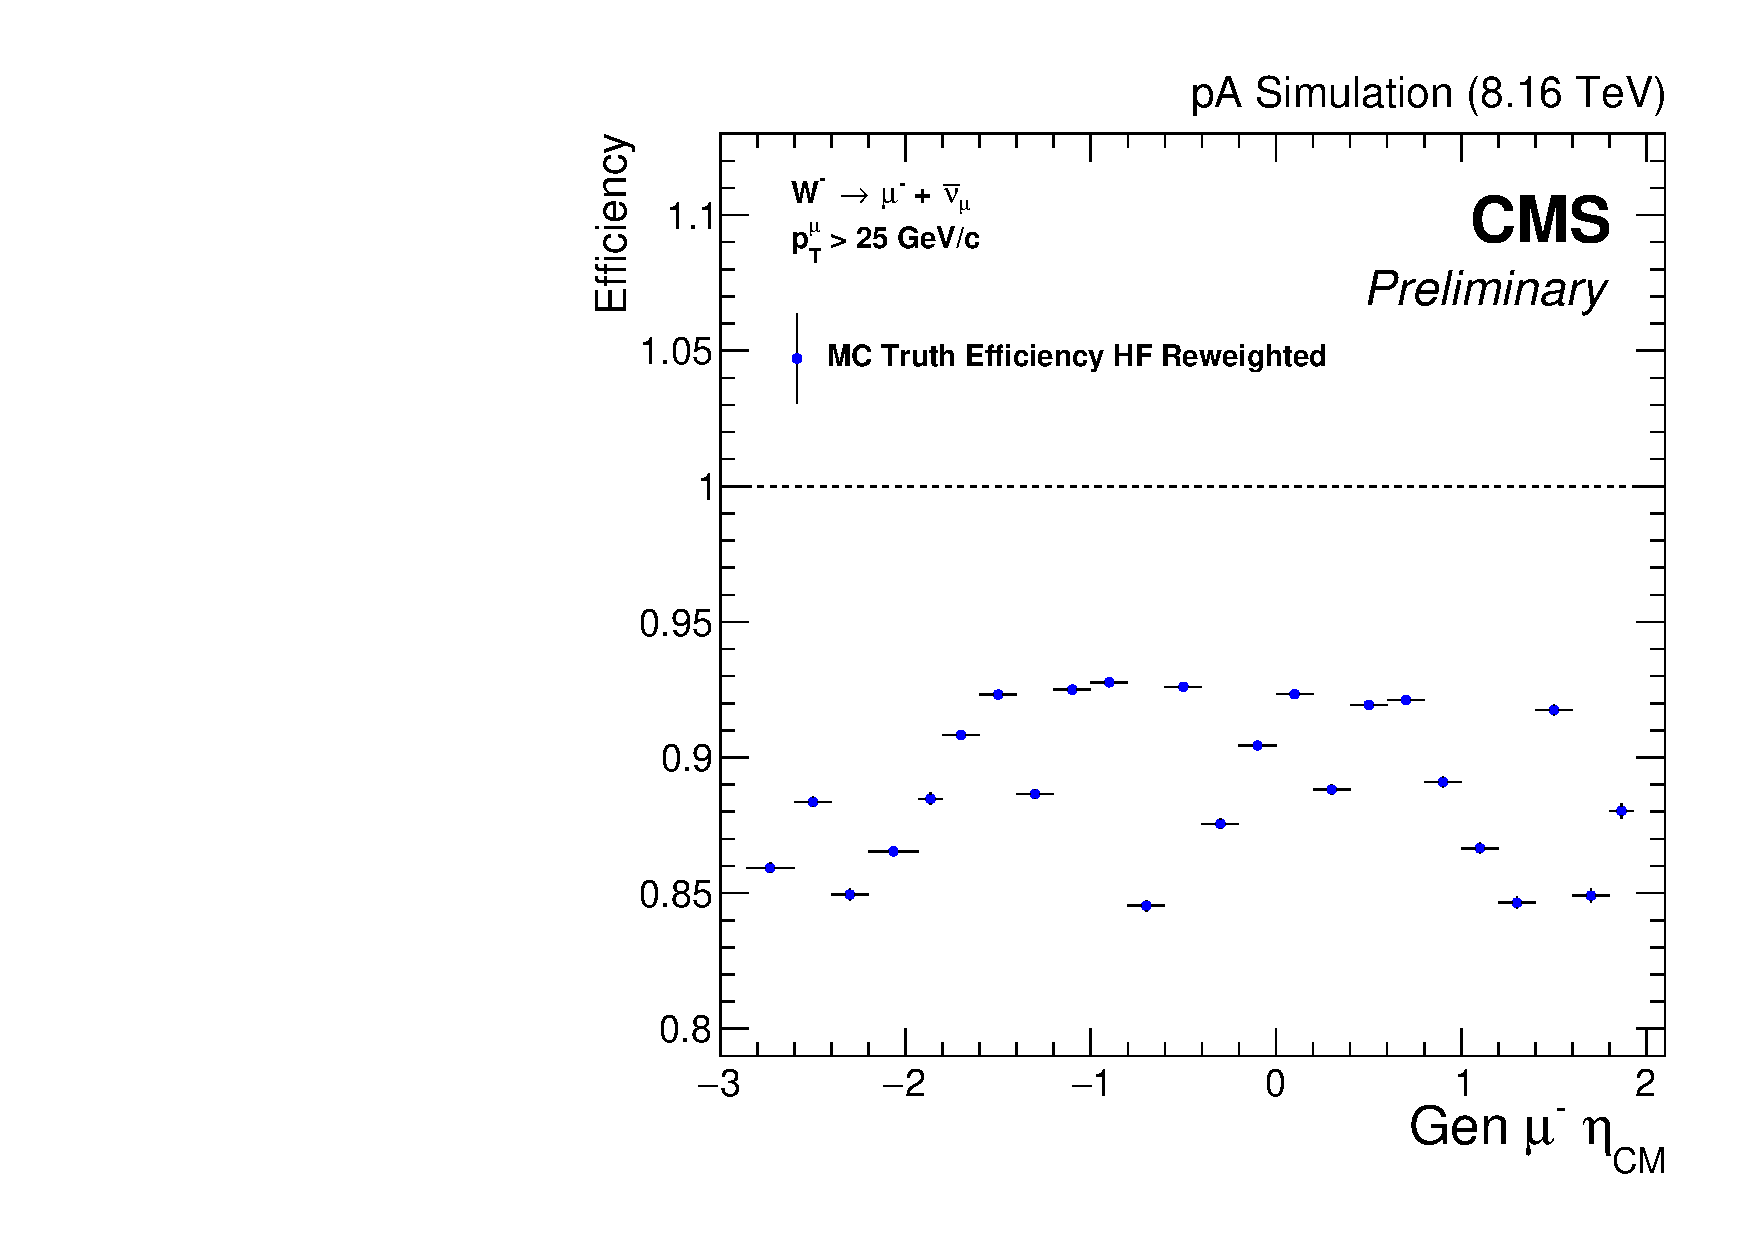
\includegraphics[width=0.45\textwidth]{Figures/WBoson/Analysis/Efficiency/Muon/PA/eff1D_EtaCM_MC_WToMuNu_PA_Minus_Total_HFCorrOnly}
   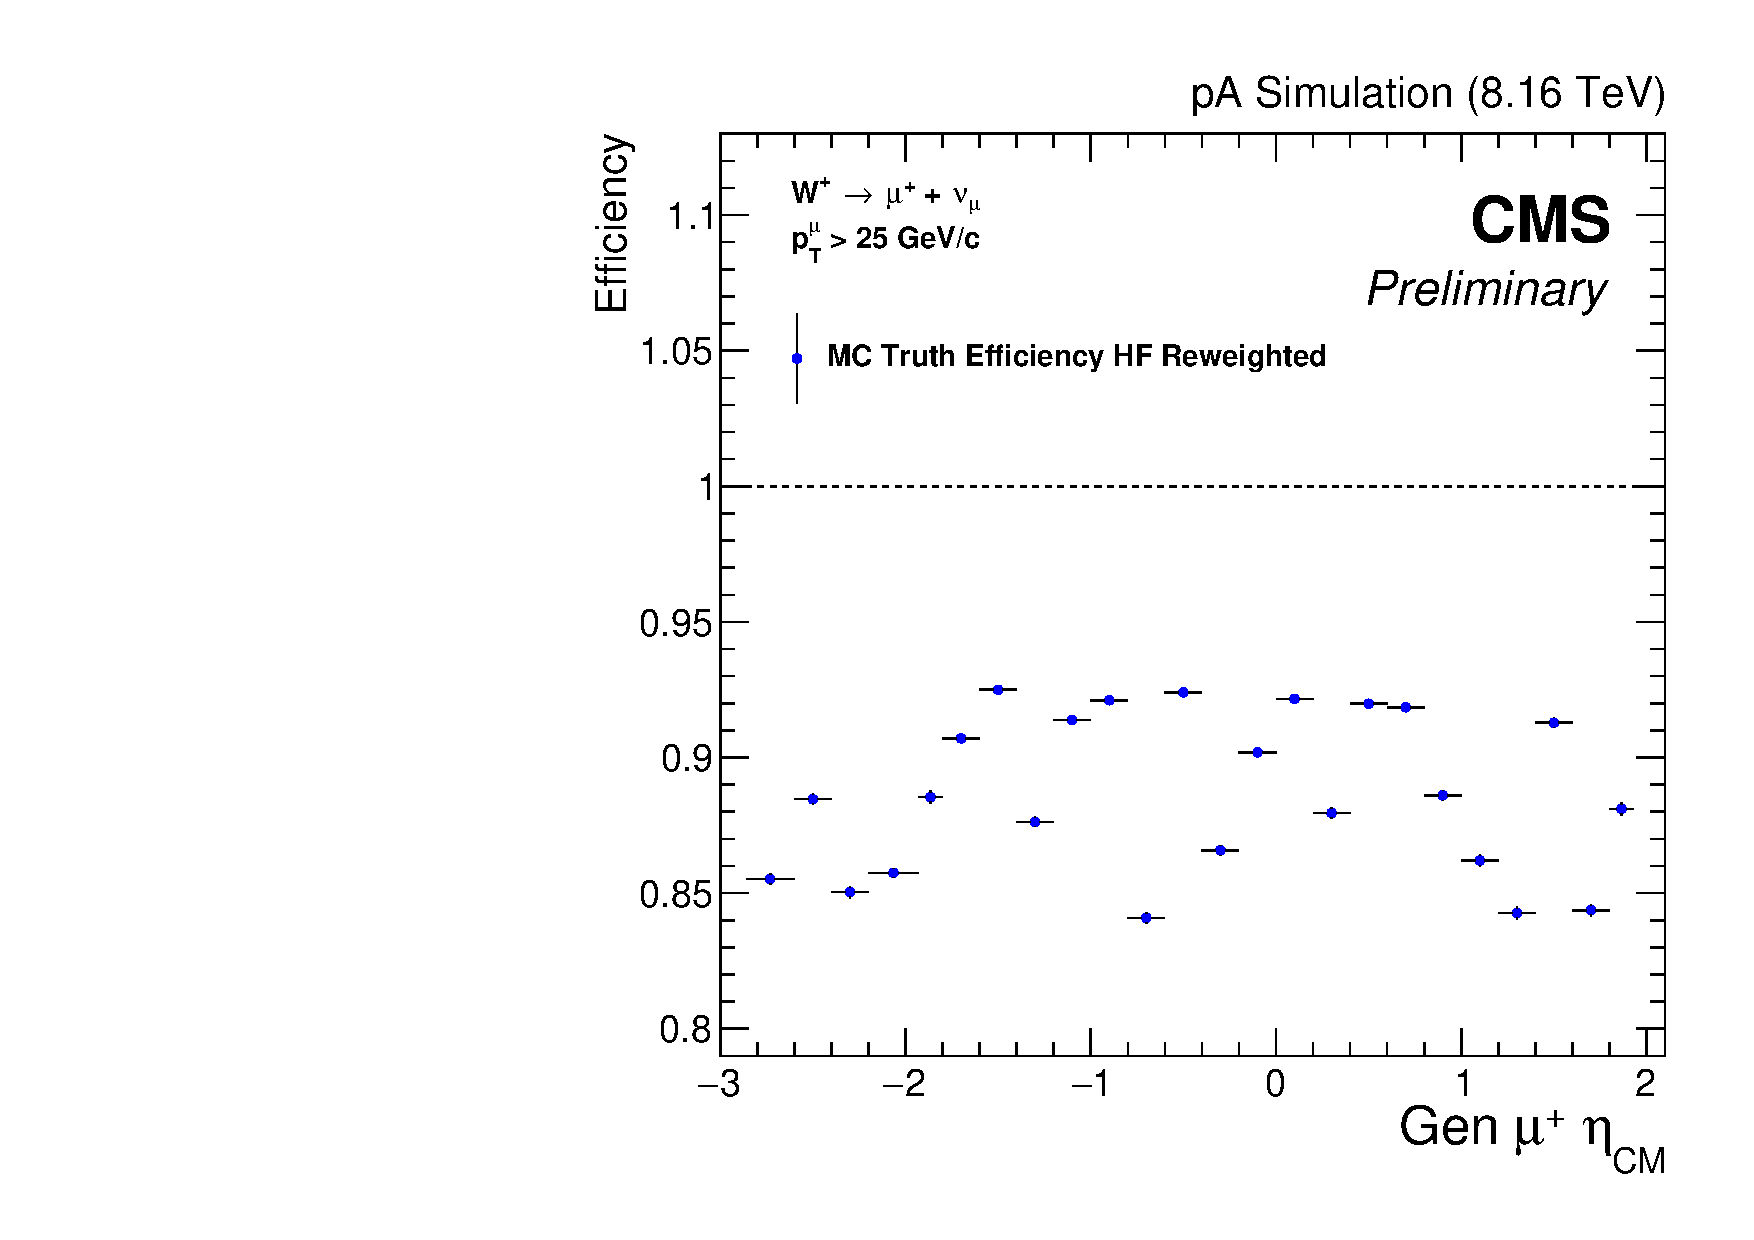
\includegraphics[width=0.45\textwidth]{Figures/WBoson/Analysis/Efficiency/Muon/PA/eff1D_EtaCM_MC_WToMuNu_PA_Plus_Total_HFCorrOnly}
 \end{center}
 \caption{Truth efficiency derived from \WToMuNu\ NLO MC sample as a function of the generated muon $\eta_{CM}$, separated in negative (left) and positive (right) charged muons. The event activity of the MC samples have been reweighed. Plots corresponds to \eq{eq:MCTruthEfficiency}, and the \RunpPb and \RunPbp MC efficiencies are combined according to \eq{eq:MCEfficiencyPA}. Only MC statistical errors are included.}
 \label{fig:MCTruthEfficiency}
\end{figure}

\subsection{Corrected muon efficiency}\label{sec:WBoson_Efficiency_CorrectedEfficiency}

The simulation of the CMS detector is very precise but still far from fully describing all the detector conditions observed in real data. In order to compensate for the imperfections in the simulations, the muon MC efficiency is corrected by applying a set of muon scale factors derived using the Tag-and-Probe method~\cite{Muon_TnP}.

The Tag-and-Probe (TnP) method is a data-driven technique widely used to compute efficiencies of physical objects, such as muons, produced from known mass resonances (e.g. \JPsi, \Z boson). One advantage of the TnP method is that it can be applied to both MC and real data, allowing to asses the differences between the data and MC efficiencies. For high \pt muons ($\pt > 15$~\GeVc), the \ZToMuMu decays are used to build a clean sample. In each event, one muon is classified as the "tag" if it has a $\pt > 15$~\GeVc and passes all the analysis cuts (trigger matching, isolation and identification), ensuring that it is a real muon, while the remaining muon is labelled as the "probe". Subsequently, the invariant mass distribution of the tag-probe dimuons is fitted in three cases: all pairs, failed pairs and passing pairs, depending on wether the probe muon passes or fails the selection criteria. The efficiency is calculated as a function of the probe \pt and $\eta_{LAB}$ in the laboratory frame by dividing the extracted yields of the passing pairs over all the pairs for various kinematic ranges of the probe. Finally, the TnP efficiencies in data and MC are compared, and the ratio of the two efficiencies is used to correct the simulations. More information about the \pPb TnP scale factors can be found in \cite{Muon_TnP_pPb}.

In this case, the muon efficiencies derived in \sect{sec:WBoson_Efficiency} are corrected by applying event by event the TnP scale factors as a function of muon $\eta_{LAB}$ and \pt. The statistical and systematic components of the TnP correction uncertainties are derived by applying the following set of variations:

\begin{enumerate}
   \item TnP statistical uncertainty:
   \begin{enumerate}
      \item For muon ID and isolation: 100 scale factor variations derived from toy MC.
      \item For trigger: Up and down $1 \sigma_{stat}$ variations.
   \end{enumerate}
   \item TnP systematic uncertainty:
   \begin{enumerate}
      \item For muon ID, isolation and trigger: Up and down by $1 \sigma_{syst}$ variations.
      \item For muon ID and isolation: Using the scale factor from the Data/MC bins instead of the one derived from fitting the ratio.
      \item For isolation: An uncertainty of {\bf 0.34\%} to account for the impact on the isolation efficiency of the different level of activity and pile-up between data and MC.
      \item For stand-alone muon reconstruction: An uncertainty of {\bf 0.6\%} to account for mismodelings in the STA efficiency.
   \end{enumerate}
\end{enumerate}

The uncertainties on the muon efficiency due to the TnP corrections are calculated in three different ways, as explained below.

\begin{enumerate}
   \item Taking the RMS between the 100 efficiencies corrected using the toy MC scale factors. Used in 1.a.
   \item Taking the maximum difference between the efficiency corrected using the nominal and the varied TnP scale factors. Used in 1.b, 2.a and 2.b.
   \item Applying the TnP scale factor uncertainty as a relative uncertainty on the corrected efficiency. Used in 2.c and 2.d.
\end{enumerate}

The total TnP uncertainty is obtained by summing in quadrature all the statistical and systematic TnP uncertainties. The TnP corrected efficiencies including their total uncertainties are shown in \fig{fig:CorrEfficiency}.

\begin{figure}[htb!]
 \begin{center}
  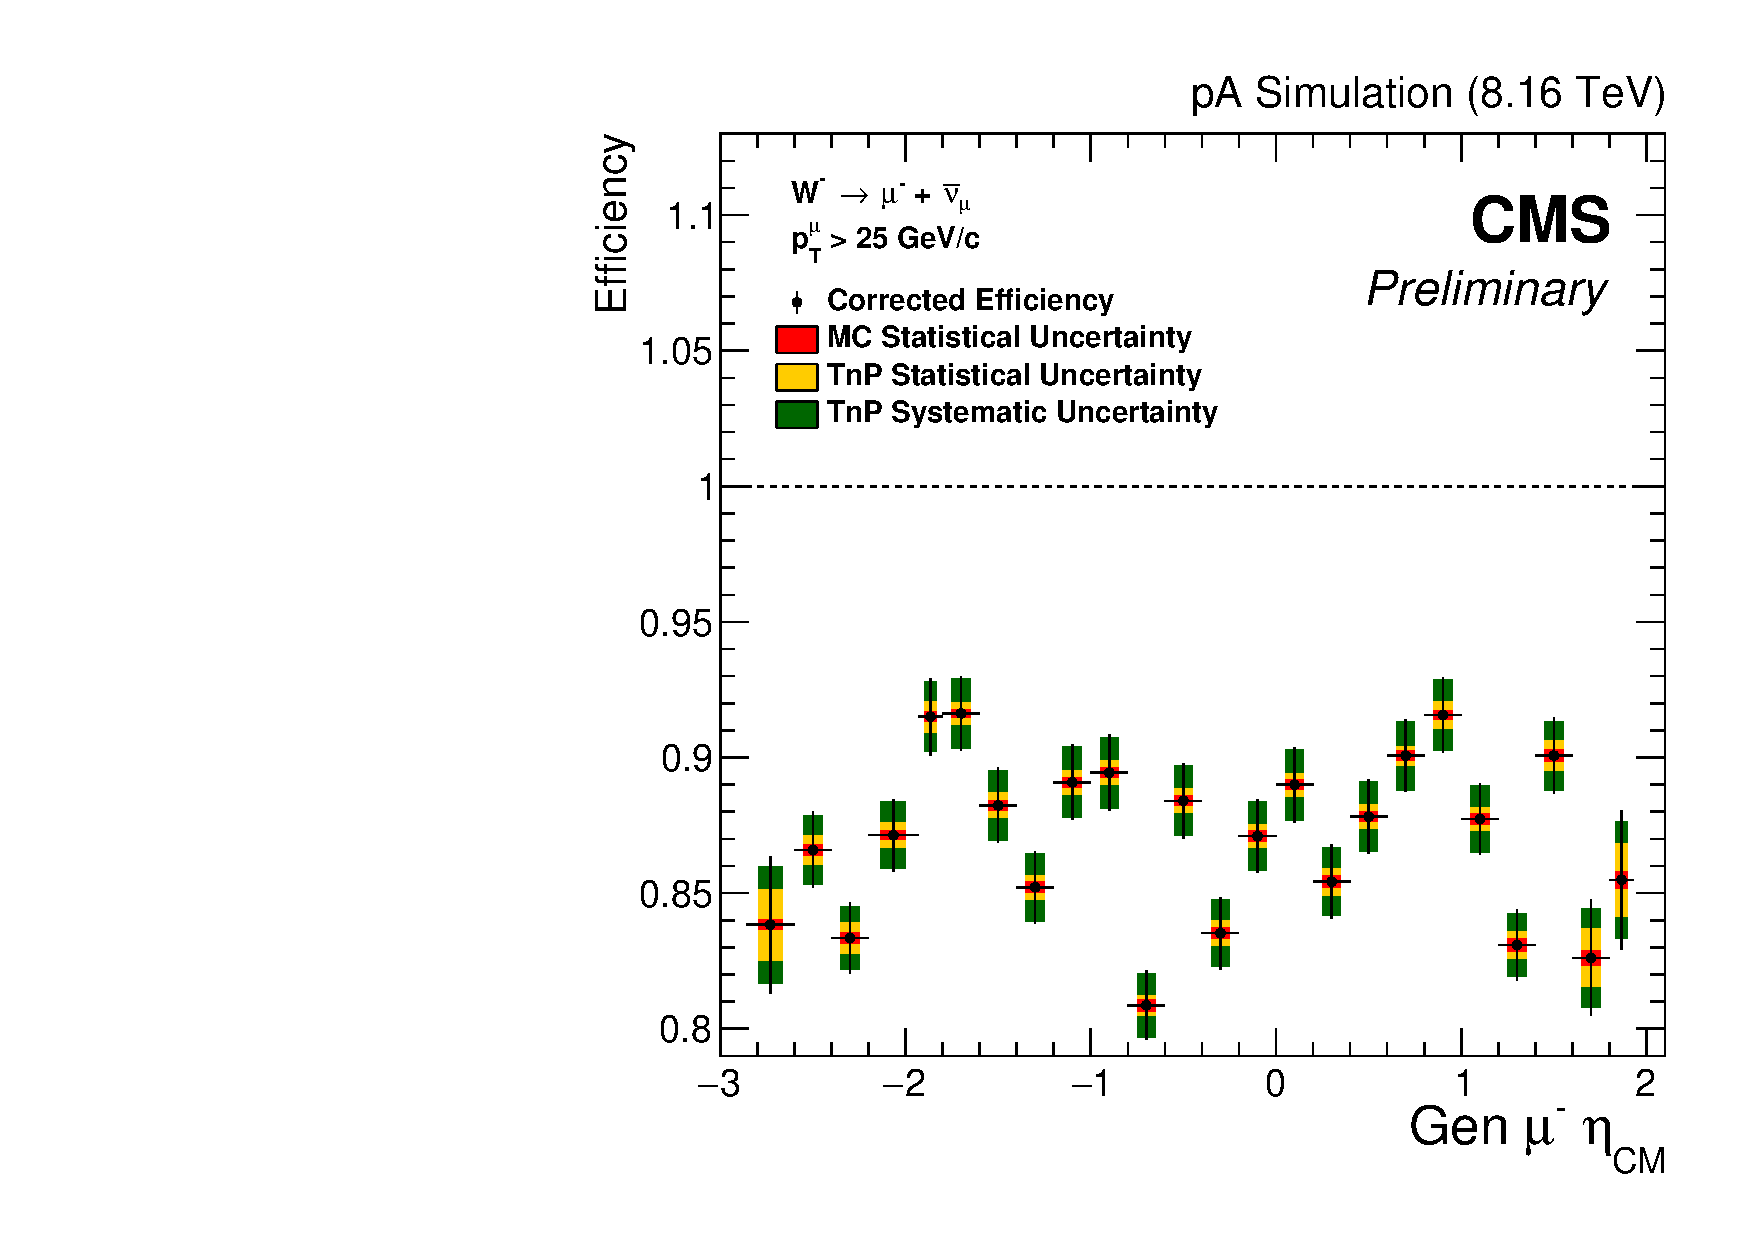
\includegraphics[width=0.45\textwidth]{Figures/WBoson/Analysis/Efficiency/Muon/PA/eff1D_EtaCM_MC_WToMuNu_PA_Minus_Total_TnP_Nominal}
  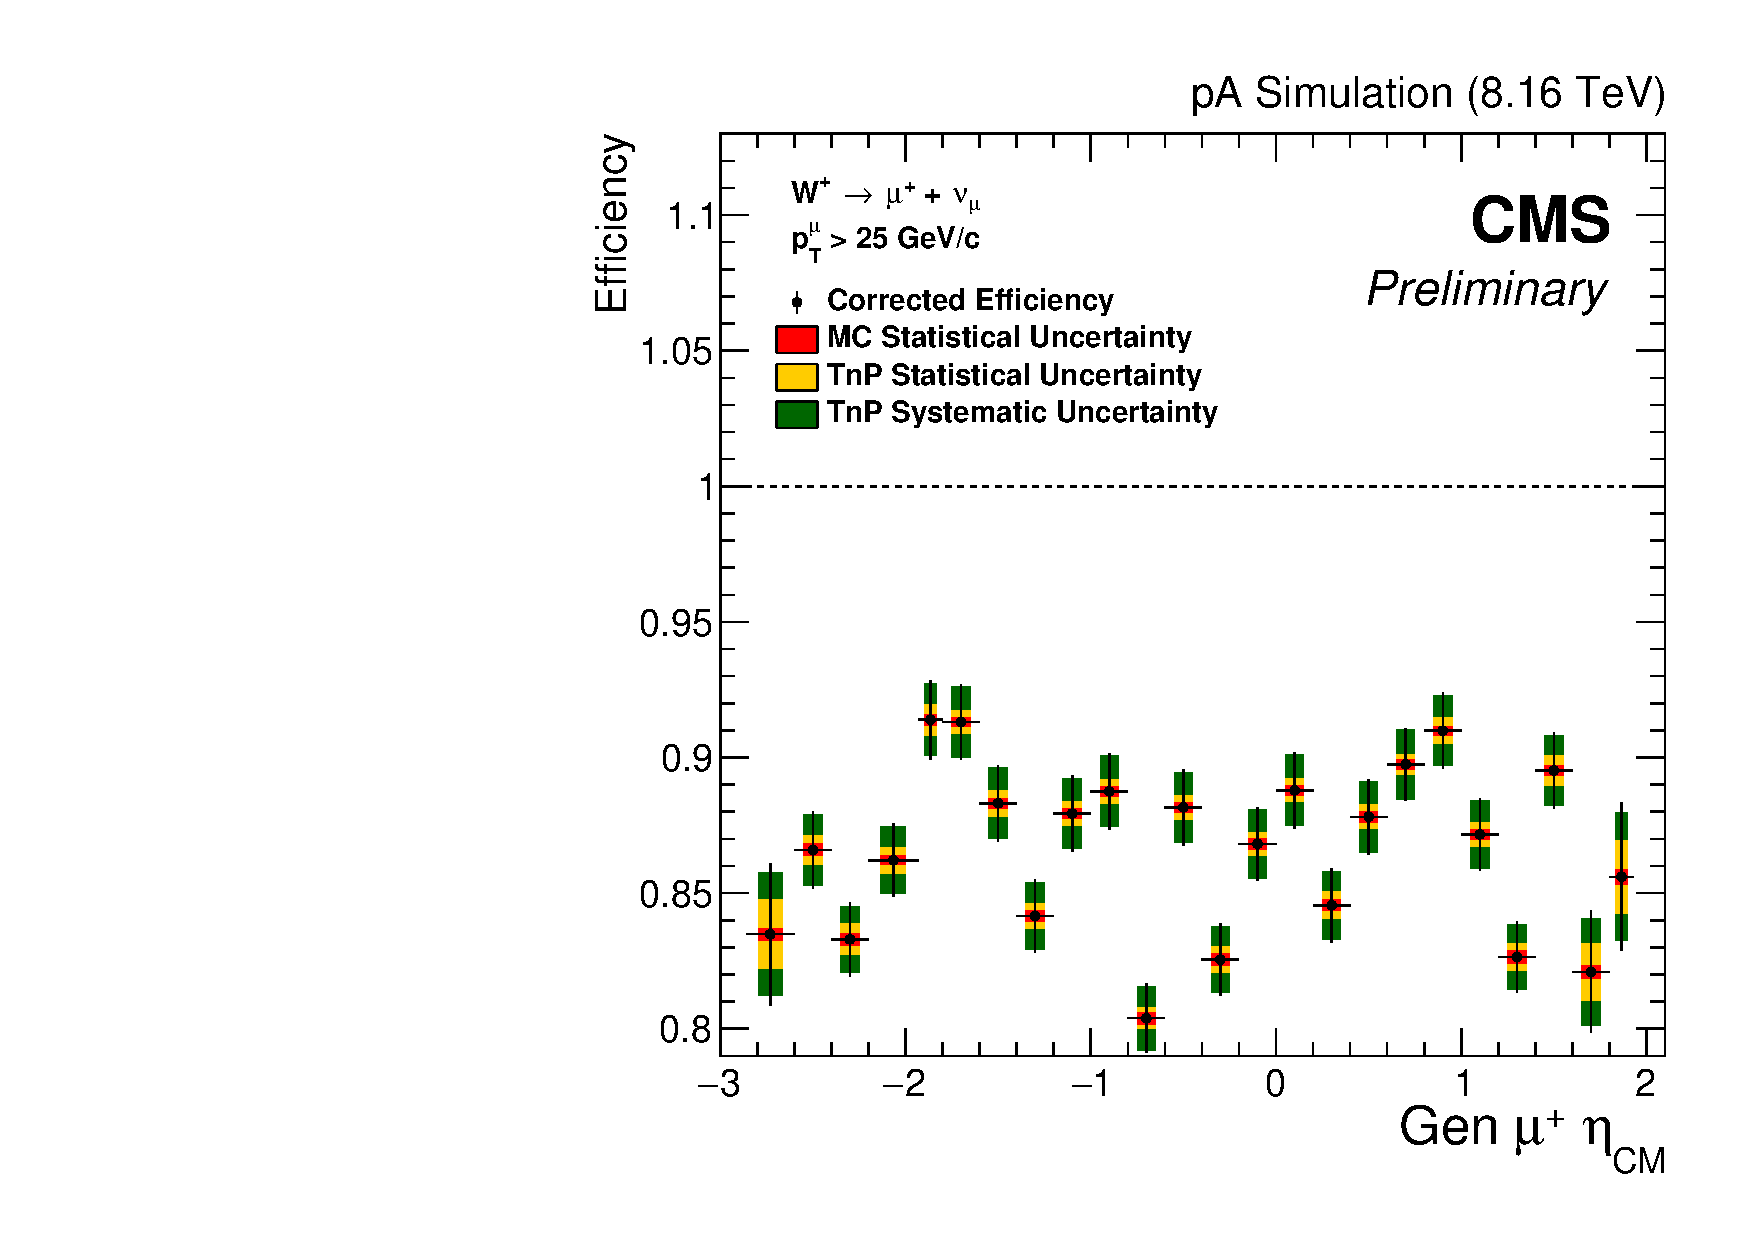
\includegraphics[width=0.45\textwidth]{Figures/WBoson/Analysis/Efficiency/Muon/PA/eff1D_EtaCM_MC_WToMuNu_PA_Plus_Total_TnP_Nominal}
 \end{center}
 \caption{Muon corrected efficiency derived from \WToMuNu \POWHEG MC sample as a function of the generated muon $\eta_{CM}$, separated in negative (left) and positive (right) charged muons. The muon efficiency has been corrected by applying the Tag and Probe scale factors event by event. The red, yellow and green boxes represents the uncertainty on the efficiency due to the MC statistics, TnP statistics and TnP systematics, respectively. The \RunpPb and \RunPbp MC efficiencies are combined according to \eq{eq:MCEfficiencyPA}.}
 \label{fig:CorrEfficiency}
\end{figure}


% END OF SUBSECTION
